\section{Geometric Meaning of Scalar Multiplication}

\begin{outcome}

\begin{enumerate}

\item[A.] Understand scalar multiplication, geometrically.

\end{enumerate}
\end{outcome}

Recall that the point $P=\left( p_{1},p_{2},p_{3}\right) $ determines
a vector $\vect{p}$ from $0$ to $P$. The length of $\vect{p}$, denoted $\vectlength
\vect{p} \vectlength $, is equal to $
\sqrt{p_{1}^{2}+p_{2}^{2}+p_{3}^{2}}$ by Definition \ref{def:distancebetweenpoints}.  

Now suppose we have a vector $\vect{u} = \leftB 
\begin{array}{lll}
u_1 &  u_2 & u_3 
\end{array}
\rightB^T$ and we multiply $\vect{u}$ by a
scalar $k$. By Definition \ref{def:vectorscalarmultiplication},
$k\vect{u} = \leftB
\begin{array}{rrr}
ku_{1} & ku_{2} & ku_{3}
\end{array}
\rightB^T $. 
Then, by using Definition \ref{def:distancebetweenpoints}, the length of this vector is given by 
\begin{equation*}
\sqrt{\left( \left( k u_{1}\right) ^{2}+\left( k u_{2}\right)
^{2}+\left( k u_{3}\right) ^{2}\right) }=\left\vert k \right\vert
\sqrt{u_{1}^{2}+u_{2}^{2}+u_{3}^{2}}
\end{equation*}
Thus the following holds.
\begin{equation*}
\vectlength k \vect{u} \vectlength =\left\vert k \right\vert
\vectlength \vect{u} \vectlength 
\end{equation*}
In other words, multiplication by a scalar magnifies or shrinks the length
of the vector by a factor of $\left\vert k \right\vert$. If $\left\vert k \right\vert > 1$, the length of the resulting vector will 
be magnified. If $\left\vert k \right\vert <1$, the length of the resulting vector will shrink. Remember that by the definition 
of the absolute value, $\left\vert k \right\vert >0$. 

What about the direction? Draw a picture of $\vect{u}$ and $k\vect{u}$
where $k$ is negative. Notice that this causes the resulting vector
to point in the opposite direction while if $k >0$ it preserves the
direction the vector points. Therefore the direction can either
reverse, if $k < 0$, or remain preserved, if $k > 0$.

Consider the following example.

\begin{example}{Graphing Scalar Multiplication}{graphingscalarmult}
Consider the vectors $\vect{u}$ and $\vect{v}$ drawn below. 

\begin{center}
\begin{tikzpicture}[scale=2]
\draw[->, thick, blue] (0,0)--(2,1);
\draw[->, thick, red] (4,1)--(5,0.5);
\node[below] at (1,1.25){$\vect{u}$};
\node[above right] at (4.5, 0.75){$\vect{v}$};
\end{tikzpicture}
\end{center}

Draw  $-\vect{u}$, $2\vect{v}$, and $-\frac{1}{2}\vect{v}$.
\end{example}

\begin{solution}

In order to find $-\vect{u}$, we preserve the length of $\vect{u}$ and simply reverse the direction.
For $2\vect{v}$, we double the length of $\vect{v}$, while preserving the direction. Finally 
$-\frac{1}{2}\vect{v}$ is found by taking half the length of $\vect{v}$ and reversing the direction. 
These vectors are shown in the following diagram. 

\begin{center}
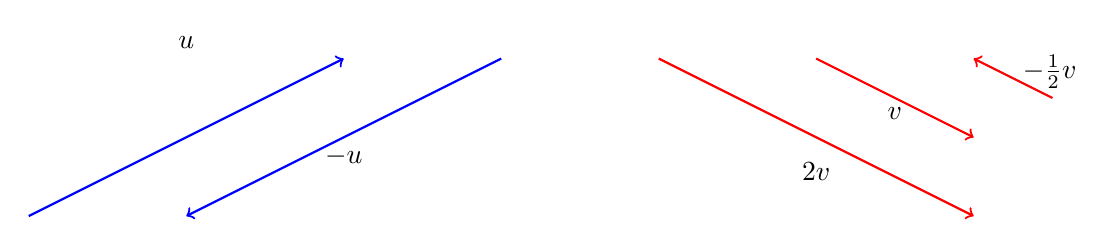
\begin{tikzpicture}[scale=2]
\draw[->, thick, blue] (0,0)--(2,1);
\draw[->, thick, blue] (3,1)--(1,0);
\draw[->, thick, red] (5,1)--(6,0.5);
\draw[->, thick, red] (6.5,0.75)--(6,1);
\draw[->, thick, red] (4,1)--(6,0);
\node[above] at (1,1){$\vect{u}$};
\node[below] at (2,0.5){$-\vect{u}$};
\node[below] at (5.5, 0.75){$\vect{v}$};
\node[above right] at (6.25, 0.75){$-\frac{1}{2}\vect{v}$};
\node[below] at (5, 0.4){$2\vect{v}$};
\end{tikzpicture}
\end{center}

\end{solution}

Now that we have studied both vector addition and scalar multiplication, we can combine the two actions. Recall 
Definition \ref{def:linearcombination} of linear combinations of vectors. We can apply this definition to 
vectors in $\mathbb{R}^n$. A linear combination of vectors in $\mathbb{R}^n$ is a sum of vectors multiplied by scalars.

In the following example, we examine the geometric meaning of this concept. 

\begin{example}{Graphing a Linear Combination of Vectors}{graphinglinearcombination}
Consider the following picture of the vectors $\vect{u}$ and $\vect{v}$

\begin{center}
\begin{tikzpicture}[scale=2]
\draw[->, thick, blue] (0,0)--(2,1);
\draw[->, thick, red] (4,1)--(5,0.5);
\node[below] at (1,1.25){$\vect{u}$};
\node[above right] at (4.5, 0.75){$\vect{v}$};
\end{tikzpicture}
\end{center}

Sketch a picture of $\vect{u}+2\vect{v},\vect{u}-\frac{1}{2}\vect{v}.$
\end{example}

\begin{solution}
The two vectors are shown below.

\begin{center}
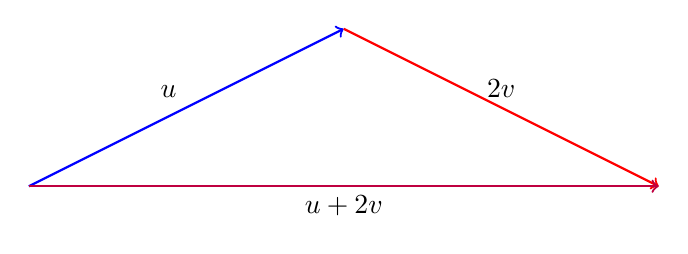
\begin{tikzpicture}[scale=2]
\draw[->, thick, blue] (0,0)--(2,1);
\draw[->, thick, red] (2,1)--(4,0);
\draw[->, thick, purple](0,0)--(4,0);
\node[above left] at (1,0.5){$\vect{u}$};
\node[above] at (3,0.5){$2\vect{v}$};
\node[below] at (2,0){$\vect{u}+2\vect{v}$};
\end{tikzpicture}
\end{center}
\begin{center}
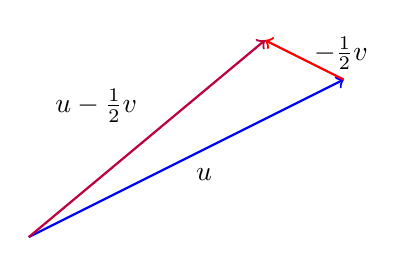
\begin{tikzpicture}[scale=2]
\draw[->, thick, blue] (0,0)--(2,1);
\draw[->, thick, red] (2,1)--(1.5, 1.25);
\draw[->, thick, purple](0,0)--(1.5,1.25);
\node[below right] at (1,0.5){$\vect{u}$};
\node[above right] at (1.75,1){$-\frac{1}{2}\vect{v}$};
\node[below left] at (0.75, 1){$\vect{u} - \frac{1}{2}\vect{v}$};
\end{tikzpicture}
\end{center}
\end{solution}